\section{Reduce MPI Synchronisation}


\chapterDescription
  {
    Around 60 minutes.
  }
  {
    A working MPI code.
  }


Peano has very strong constraints on the master-worker and worker-master
communication as the data exchange between these two is synchronous. It imposes
a partial order. If that slows down your application (you see this from the
mpianalysis reports), you can kind of weaken the communication constraints. 
Often, some data is not required immediately, not required globally all the
time, or doesn't have to be 100\% correct at all algorithmic stages. This
chapter discusses some things that you can do then.

On the following pages, we assume that you have proper load balancing.


\subsection{The smell}

Strong synchronisation materialises in very regular patterns where each rank
waits for rank 0 to start up a new traversal.

\begin{center}
  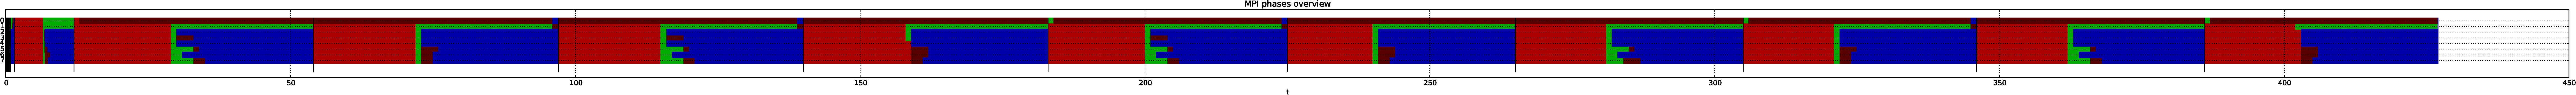
\includegraphics[width=0.9\textwidth]{43_mpi-synchronisation/mpi-phases-before.pdf}
\end{center}

It also becomes obvious if you study how often a master has to work for its 
workers. 
In the picture below, only rank 0 synchronises the other ranks.
In this case, you have to weaken the global synchronisation.
If multiple of these edges pop up, it is time to weaken all the worker-master
synchronisations---unless you can identify that you have a load balancing issue.


\begin{center}
  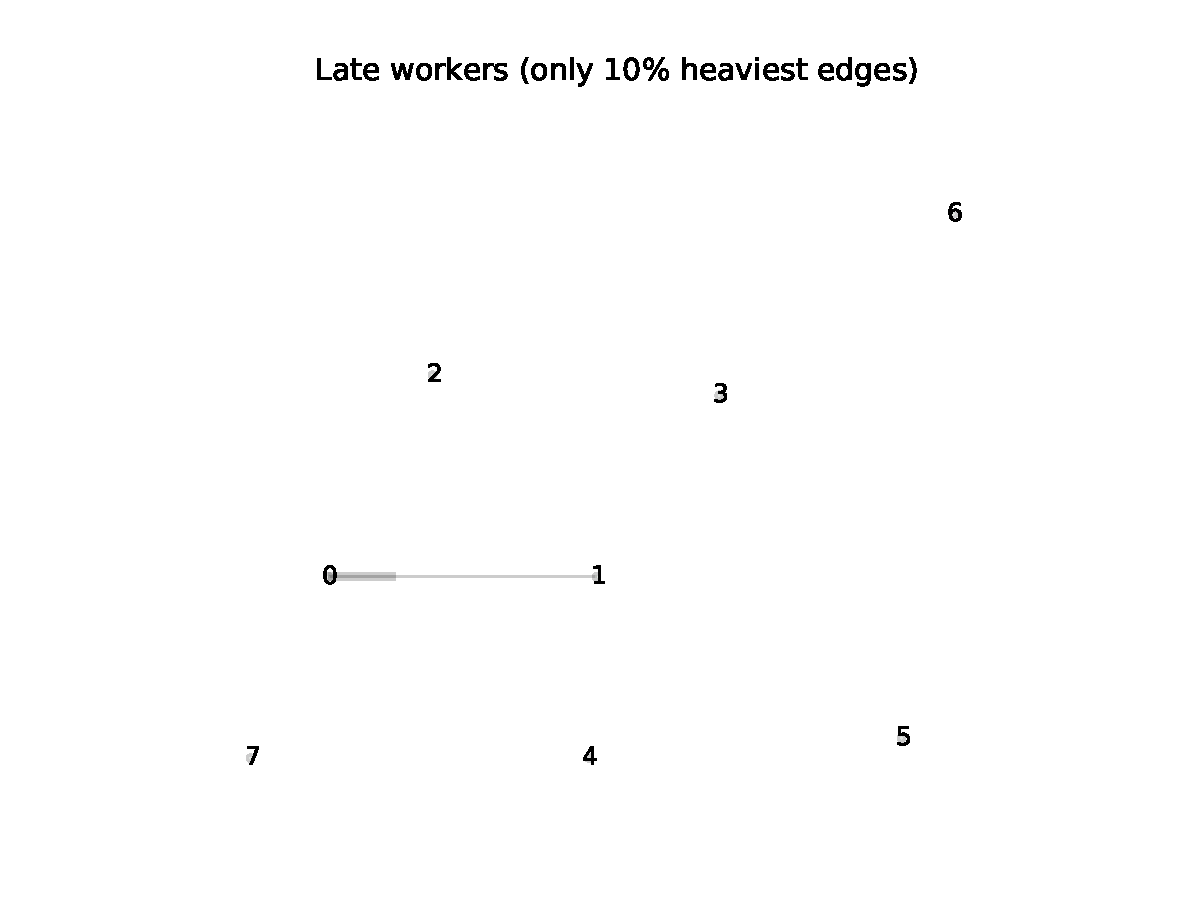
\includegraphics[width=0.5\textwidth]{43_mpi-synchronisation/master-worker-before.pdf}
\end{center}


\subsection{Weaken synchronisation with global master}

The global master (rank 0) is kind of a pulse generator for the whole code. 
Whenever the \texttt{runAsMaster} operation triggers \texttt{iterate}, it tells
each rank that handles a partition which adapter to use and to start its
traversal or wait for its master to trigger the traversal, respectively.
This is a very strong synchronisation.
Notably, no rank can continue to work with the next iteration unless rank 0 runs
into the next \texttt{iterate} as well.
There are basically two variants to improve this situation:

\begin{enumerate}
  \item Perform more than one time step with the same adapter and settings in a
  row. For this, use the integer argument of \texttt{iterate()}. Note that
  running multiple time steps switches off load balancing for this phase of the program.
  Obviously, this version works if and only if you run the same adapter several 
  times.
  \item You may alternatively find out that you don't need the rank 0 (that
  doesn't hold any data anyway) to wait for all the other ranks in each
  iteration. Often, you run for example a sequence of adapters and you require
  global data (such as global residual) only after the last run. 
  If you want to realise the second variant, you have to ensure that all
  mappings you use (also the predefined ones) return false in
  \texttt{prepareSendToWorker(...)}.
\end{enumerate}




\subsection{Postpone master-worker and worker-master data exchange}
    Take the communication specification of each mapping. By default, they are set to the most general case. Adopt it to your algorithmic needs (see documentation of the communication specification class)/


Introduce eager send and late receive

By default, Peano send away data from a local node if and only if it has traversed the whole local tree. In return, it requires all input data before it starts to traverse anything. You may want to tailor this to your needs and send data earlier and receive data later which allows you to overlap computations more aggressively. To do so, you have to adopt the communication specification fields of your mappings. See the documentation of the underlying class for more details.
Avoid communication with rank 0


\subsection{Skip worker-master data transfer locally/sporadically}
